%Beamer class
\documentclass{beamer}

\usepackage[czech]{babel}
\usepackage[cp1250]{inputenc}
\usepackage{fontenc}
\usepackage{tgheros}
\usepackage{array}
\usepackage{color}
\usepackage{hyperref}

\usetheme{Antibes}
\usecolortheme{crane}


\title[BE1M13VES]{BE1M13VES}
\subtitle[Manufacturing of Electrical Components] {Manufacturing of Electrical Components}
\author[Brejcha]{Michal Brejcha}
\institute[CTU]{CTU in Prague}
\date[Prague, 2017]{Prague, 2017}

\begin{document}
%------------------------------------------------------------------------------
%Uvodni slajd
%------------------------------------------------------------------------------
\frame{\titlepage}

\begin{frame}
\frametitle{Overview} 
\tableofcontents
\end{frame}

\AtBeginSection[]
{
  \begin{frame}
    \frametitle{TOPIC}
    \tableofcontents[currentsection]
  \end{frame}
}

%------------------------------------------------------------------------------
%Frquency dependency of resistors
%------------------------------------------------------------------------------
\section{\texorpdfstring{Semiconductor Components}{Semiconductor Components}}
%------------------------------------------------------------------------------
	\begin{frame}
    \frametitle{Semiconductor Components}
		\textbf{Basic properties}
		\begin{itemize}
		\item Nonlinear characteristics - used for rectifying, sensing, saturation etc.
		\item VA characteristics are quite dependent on ambient factors - temperature, light.
		\item Some components are able to amplify the input signal - transistors
		\end{itemize}
		
	\end{frame}
%------------------------------------------------------------------------------
	\begin{frame}
    \frametitle{Doping}
		\small
		\textbf{Intrinsic semiconductors (semiconductors without impurities):}
		
		\begin{itemize}
			\item The free charge is excited via temperature or light.
			\item Quite small conductivity dependent on ambient factors.
		\end{itemize}
		
		\textbf{Extrinsic semiconductors (semiconductors with doped material):}
		
		\begin{itemize}
			\item Most of the free charge is excited at room temperature from impurities.
			\item Similar behavior as metal conductors (rising resistance with temperature).
			\item Two types of doped materials (dopants): \textbf{\textcolor{brown}{donors \& acceptors}}
		\end{itemize}
		
	\end{frame}
%------------------------------------------------------------------------------
	\begin{frame}
    \frametitle{Doping}
		\small
		
		\textbf{Degenerate semiconductors}
		
		\begin{itemize}
			\item High level of dopant.
			\item Almost the same behaviour as metal conductors.
			\item Their are used to create contact layer between metal wire and semiconductor.
		\end{itemize}
	\end{frame}
%------------------------------------------------------------------------------
	\begin{frame}
    \frametitle{Temperature dependency}
		%\begin{center}
			%\begin{tabular}{m{0.45\linewidth} m{0.45\linewidth}}
			%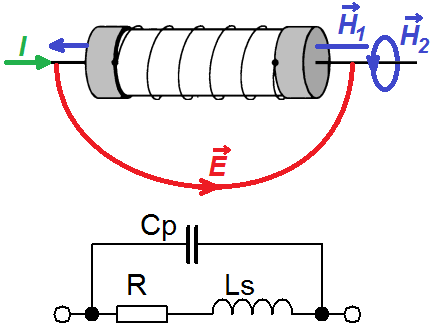
\includegraphics[scale=0.4]{obr01_poleRes.png} &
			%
			%\begin{itemize}
				%\item $H_1$, $H_2$... magnetic field from resistive track and leads.
				%\item $E$... electric field (capacitance) between opposite sides of package and leads.
			%\end{itemize}
			%\end{tabular}
		%\end{center}
	\end{frame}
%------------------------------------------------------------------------------
%Frquency dependency of resistors
%------------------------------------------------------------------------------
\section{\texorpdfstring{Light Dependent Resistor}{Light Dependent Resistor}}
%------------------------------------------------------------------------------
	\begin{frame}
    \frametitle{LDR, Photoresistor - Basic properties}
		\small
		\begin{itemize}
		\item The resistance decreases with illumination.
		\item The spectral light sensitivity depends on semiconductor material.
		%\item No PN junction:
			%\begin{itemize}
				%\item intrisic - high resistance, sensitive to short wavelengths of light
				%\item extrinsic - smaller resistance, sensitive to longer vawelenghts of light (IR)
			%\end{itemize}
		\end{itemize}
		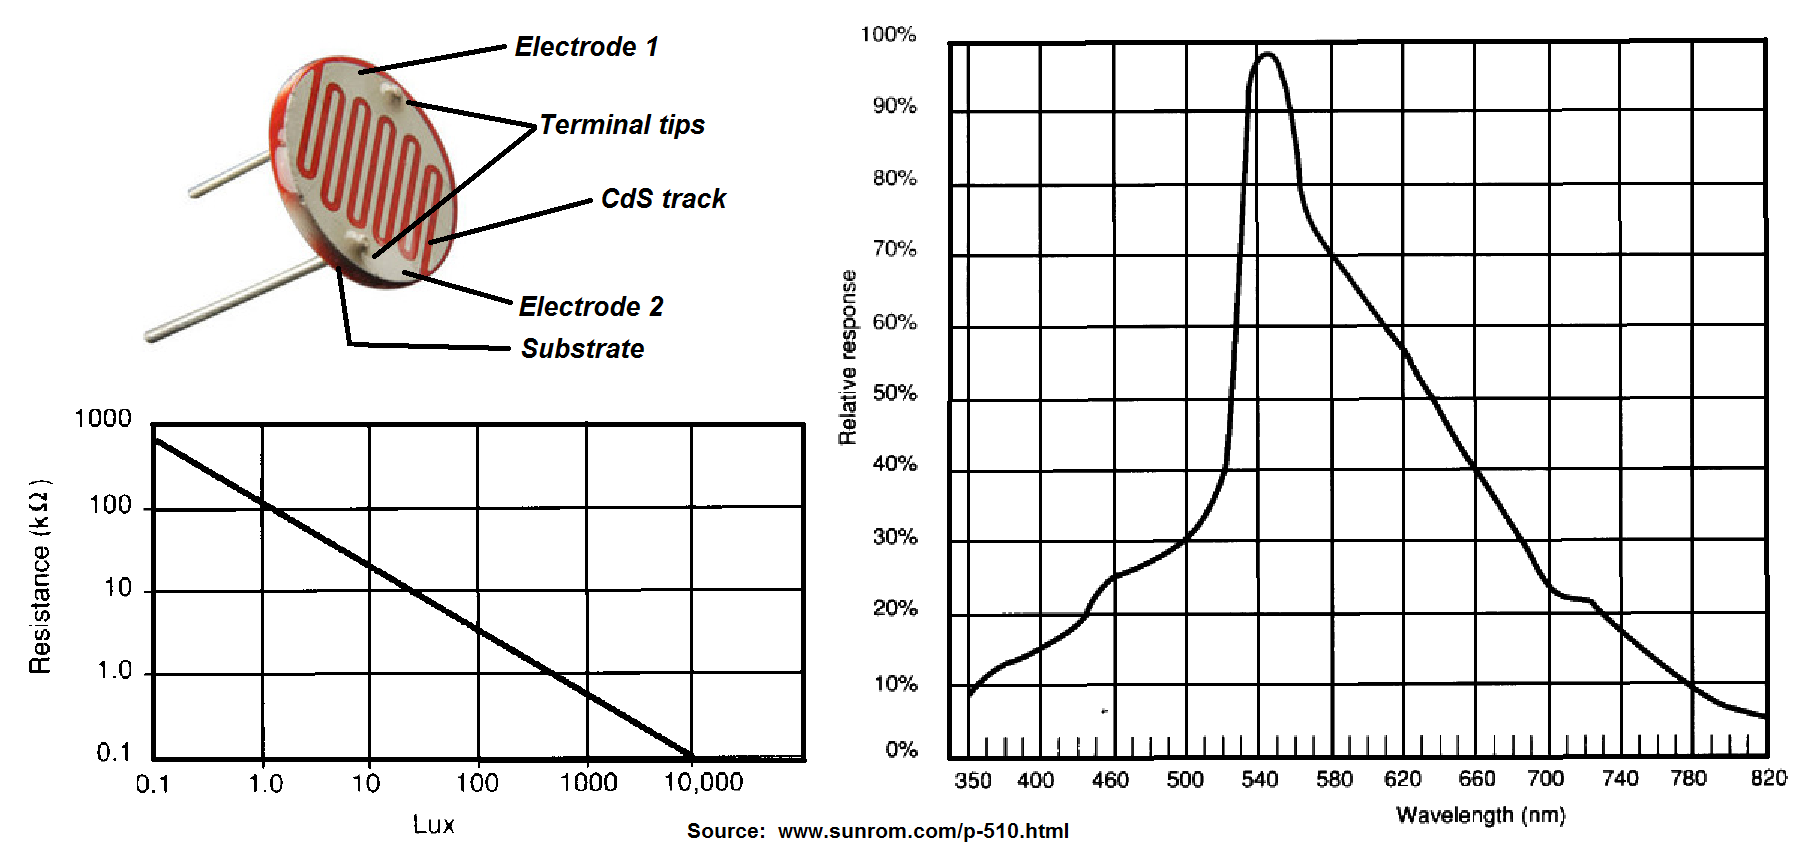
\includegraphics[scale=0.22]{obr01_fotoodpor.png}
	\end{frame}
%------------------------------------------------------------------------------
\end{document}